% Chapter 2

\chapter{Methods and Models} % Main chapter title

\label{Chapter2} % For referencing the chapter elsewhere, use \ref{Chapter1} 

\lhead{Chapter 2. \emph{Methods and Models}} % This is for the header on each page - perhaps a shortened title

%----------------------------------------------------------------------------------------

\section{Empirical functional and anatomical connectivity matrices}

\section{Randomization Methods and Network Characterizations}

\subsection{The Brain Graph}

The brain graphs are derived from the empirical fMRI-BOLD and DW-MRI data sets with the help of network science. Those data sets reflect measurements from $N=90$ brain regions, the equivalent terminology is so called "nodes" in the graph theory. The nodes can be connected to each other by means of "edges". If the graph is constructed on the fMRI-BOLD data, the edge is interpreted as the strength of functional correlation between two nodes. If the graph is built on the DW-MRI data, an existing edge is considered as the structural connectivity between two nodes. 

The brain graphs in this project are generated after binarizing the functional connectivity matrix (FCM) and anatomical connectivity matrix (ACM). Binarization here means converting all the values in a given matrix into 1's and 0's. Because of the nature of their definition, both empirical data sets have values between 0 and 1 reflecting correlation in case of FCM or probability in case of ACM. We define a threshold value, $r$, for the strength of correlations in FCM. Then, the values greater and equal to $r$ are assigned to 1, while others are set to 0. This thresholding is applied by means of the strength of probability value, $p$, for the ACM. The binarized matrix is the basis of graph construction, and it is better called as "adjacency matrix". \textit{Networkx} software package in PYTHON is used to built graphs given adjacency matrices. Neither the direction of functional or anatomical connectivity between nodes, nor any other values apart from 0 and 1  are considered in adjacency matrices, the resultant graphs are therefore classified in "undirected" and "unweighted" category. In other words, all the edges are thought to be homogeneous and it is possible to move in any direction along an edge. 

\begin{figure}[htbp]
 %\begin{tabular}{cc}
  \centering
	\includegraphics[width=0.48\textwidth]{Figures/adj_mtx.png} 
	  
  
    %\includegraphics[width=0.48\textwidth]{Figures/adj_mtx.png} &
	%\includegraphics[width=0.48\textwidth]{Figures/adj_mtx.png} \\
    
    \rule{35em}{0.5pt}
  \caption[Binarizing via thresholding]{Binarizing via thresholding).}
  \label{fig:Electron}
 %\end{tabular}	
\end{figure}


The brain graph can be reconstructed with some randomization tools, such as inspired from Erd\H{o}s-R\'{e}nyi type randomization and configuration model. The following sections will cover the randomization methods rebuilding the brain graphs and introduce some of the topological concepts identifying a graph, i.e. degree of a node, clustering coefficient etc.. The main objective of this section is to characterize brain graphs binarized via a threshold and a probability range $p,r=[0,1]$ and to compare them with the random graphs in terms of topological properties in a network.

\subsection{Erd\H{o}s-R\'{e}nyi Type Randomization}

Given total number of nodes $N$ and a probability $P$, Paul Erd\H{o}s and Alfr\'{e}d R\'{e}nyi produced an undirected graph $G(N,P)$, in which the presence of any edge between two nodes is assigned with probability $P$. 
One can generalize the total number of edges $L$ in an  Erd\H{o}s-R\'{e}nyi type random graph as the following: $\binom {N} {2}P$, pointing out a binomial distribution for the edges per node.

It is possible to improve new randomization tools with adaptations in Erd\H{o}s-R\'{e}nyi method, i.e. given $N$ and $L$, an intended graph $G(N,L)$ can be picked uniformly random out of set of all potential graphs having $N$ nodes and $L$ edges. The probability for a graph to be picked among all the others is $\frac{L}{\binom {N}{2}}  $. One can study the relevance of $G(N,P)$ and $G(N,L)$ even more detailed, but for the sake of simplicity, Erd\H{o}s-R\'{e}nyi model will not discussed further here.

\begin{figure}[htbp]
 %\begin{tabular}{cc}
  \centering
	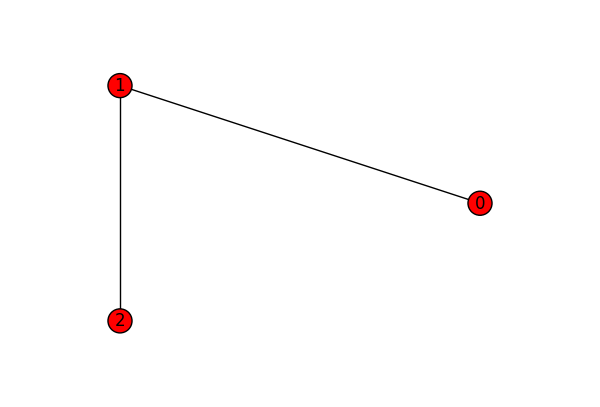
\includegraphics[width=0.30\textwidth, height=40mm]{Figures/f1.png}  
	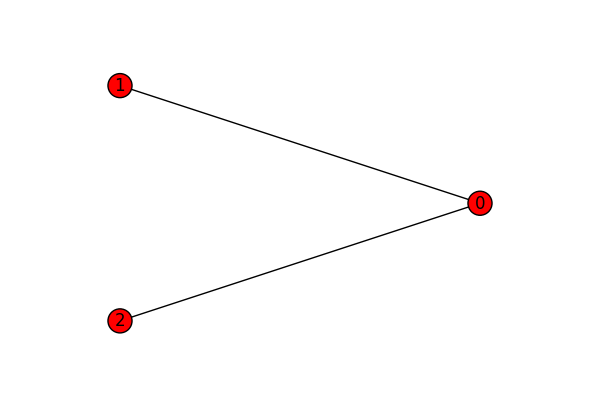
\includegraphics[width=0.30\textwidth, height=40mm]{Figures/f2.png} 
    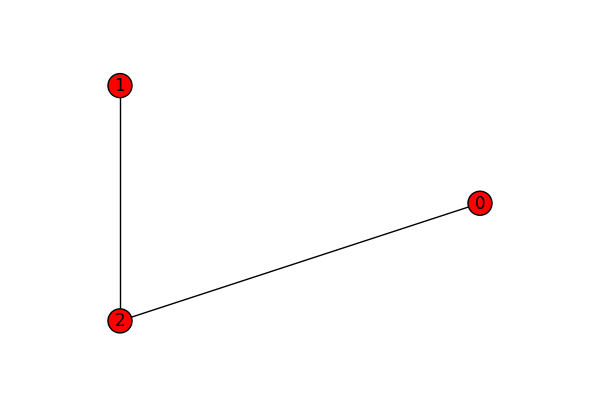
\includegraphics[width=0.30\textwidth, height=40mm]{Figures/f3.png}

    \rule{35em}{0.5pt}
  \caption[Erdos-Renyi Example]{An illustration to the set of all $G(N,L)$ type random graphs with $N=3$ and $L=2$.}
  \label{fig:Erdos-Renyi Example}
 %\end{tabular}	
\end{figure}

Figure 2.2 illustrates all possible graphs having 3 nodes ans 2 edges in total. One of those 3 simple graph is chosen uniformly random for the $G(N,L)$ randomization type means that each graph is chosen with probability $P=\dfrac{1}{3}$.  

The $G(N,L)$ type randomization is the first method used to derive random graphs from the adjacency matrices of FCM and ACM in this project. Both matrices have $N=90$ nodes, however $L$ changes at each brain graph according to the applied threshold and probability level, therefore it is always recalculated. 

\subsection{Double-Edge-Swap Type Randomization}

The \textit{degree} of a node is defined as the number of edges connected to that node, from now on it will be denoted with $k_i$ for the node $i$. The double-edge-swap method manipulates a given graph by swapping two existing edges among four nodes, while keeping the node degrees fixed. 


\begin{figure}[htbp]
 %\begin{tabular}{cc}
  \centering
	\includegraphics[width=0.30\textwidth, height=40mm]{Figures/s1.png}  
    \includegraphics[width=0.04\textwidth, height=20mm]{Figures/arrow.png}  
	\includegraphics[width=0.30\textwidth, height=40mm]{Figures/s2.png} 
    \rule{35em}{0.5pt}
  \caption[Double-Edge-Swap Example]{Swapping edges between 4 nodes}
  \label{fig:Double-Edge-Swap Example}
 %\end{tabular}	
\end{figure}

Figure 2.3 illustrates randomly chosen double edges in a sample graph to be swapped. After the existing edges are removed, the new couple of nodes are rewired. The $k_i$ of each node is the same before and after swapping. The \textit{degree distribution} of a graph is a topological property, which reveals a probability distribution of node degrees over whole graph. Although the randomly constructed graphs with the double-edge-swap method based on the brain graphs of FCM and ACM are expected to have the same degree distribution, it is not a unique property identifying a graph.

\subsection{Configuration Model Randomization}

The \textit{degree sequence} of a graph is either ascending or descending sequence of node degrees in a graph. The configuration model intends to return a random graph with given degree sequence. The ideal concept of this model is to assign edges to the nodes randomly until the desired degree sequence is matched. However, the algorithms practicing the configuration model are not so trivial due to self-loops (node is connected to itself) and parallel edges (duplicating edges), which are both undesirable graph properties in this project. 

\begin{figure}[htbp]
 %\begin{tabular}{cc}
  \centering
	\includegraphics[width=0.50\textwidth, height=60mm]{Figures/c1.png}  
    \rule{35em}{0.5pt}
    \caption[Degree Sequence Definition]{The degrees of the nodes: $k_0 = 2$, $k_1 =1$, $k_2=2$, $k_3=3$ and the degree sequence in non-increasing order in the sample graph : $\{3,\,2,\,2,\,1\}$}
  \label{fig:Degree Sequence Definition}
 %\end{tabular}	
\end{figure}

Figure 2.4 points out the relevance of degree sequence to the node degrees. It should be reminded that the degree distribution and the degree sequence are not the same metrics.  

The configuration model variant used here is the expected-degree-graph method, which has an option to exclude self-loops and parallel edges. This algorithm receives the list of expected degree sequence as input, $(k_u, k_v, k_m, k_l, ...)$, and assigns edges between nodes with a predefined probability $P_{uv}=\dfrac{k_u k_w}{\sum_{i}k_i}$. This tool does not guarantee to construct graphs with exactly the same given degree sequence but with the closest possible sequence.  

\subsection{Preserved-Degree-Distribution Type Randomization}

The \textit{degree distribution} of a network reflects the probability of a node to have a given number of degree \textit{k}. The preserved-degree-distribution method randomizes a given undirected network by rewiring its edges randomly while preserving its degree distribution. The method first chooses four target nodes randomly, then flips the edges between those nodes with the probability of $P=0.5$. The total number of rewirings to be performed is given as an iteration parameter to the method. 

 

 

\section{FitzHugh-Nagumo Model for Neuronal Activity Simulation}

\section{Balloon-Windkessel Model for BOLD Activity Simulation} 
 
%----------------------------------------------------------------------------------------
